\documentclass[10pt,twocolumn]{article}
\usepackage[utf8]{inputenc}
\usepackage[margin=1.55cm]{geometry}
\usepackage{amsmath,amssymb}
\usepackage{booktabs}
\usepackage{graphicx}
\usepackage{microtype}
\usepackage{cite}
\usepackage{enumitem}
\setlist{noitemsep,topsep=2pt,parsep=0pt,partopsep=0pt}
\usepackage[font=small,labelfont=bf,skip=3pt]{caption}
\setlength{\textfloatsep}{6pt plus 2pt minus 2pt}
\setlength{\dbltextfloatsep}{6pt plus 2pt minus 2pt}
\setlength{\floatsep}{4pt plus 2pt minus 2pt}
\setlength{\dblfloatsep}{4pt plus 2pt minus 2pt}
\usepackage{hyperref}
\hypersetup{colorlinks=true, linkcolor=blue, citecolor=blue, urlcolor=blue}

% Float placement parameters for 2-column layout
\setcounter{topnumber}{3}
\setcounter{bottomnumber}{3}
\setcounter{totalnumber}{4}
\setcounter{dbltopnumber}{2}
\renewcommand{\topfraction}{0.95}
\renewcommand{\dbltopfraction}{0.95}
\renewcommand{\textfraction}{0.05}
\renewcommand{\floatpagefraction}{0.8}
\renewcommand{\dblfloatpagefraction}{0.8}

\title{\textbf{Confidence Calibration of Small Open LLMs:\\Token Probability vs. Verbalized vs. Consistency}}
\author{
  \textbf{Mohammadreza Sharifi}\\
  \texttt{m.sharifi8080@gmail.com}
}
\date{October 2026}

\begin{document}
\maketitle

\begin{abstract}
Reliable deployment of Large Language Models (LLMs) requires trustworthy uncertainty estimation: models should exhibit high confidence when correct and low confidence when wrong. While recent literature on proprietary frontier models suggests that verbalized confidence often surpasses token probability, this empirical study investigates whether this finding holds for small open-weight instruction-tuned models (0.5B to 7B parameters). We evaluate four confidence estimation methods---token probability, verbalized 0--100 scoring, self-check P(True), and 5-sample self-consistency---across the Qwen2.5 model family on TriviaQA (open-domain QA) and SciQ (multiple-choice science QA), comprising 3,995 evaluated generations. Our results reveal a stark contrast: verbalized confidence fails systematically on small models, exhibiting mode collapse near 85--95\% confidence and near-random discriminative ability (AUROC 0.414--0.618). Conversely, length-normalized token probability and self-consistency consistently achieve high discrimination (AUROC up to 0.909) and lowest Expected Calibration Error (ECE down to 0.146), confirming that internal representation signals remain superior for small language models.
\end{abstract}

\section{Introduction}
Uncertainty quantification in Large Language Models (LLMs) is fundamental for trustworthy AI, automated decision routing, and cascading architectures where small models defer uncertain queries to larger models~\cite{zhang2026confidence}. A well-calibrated confidence metric enables systems to reliably refuse answers or query human supervisors when generation correctness is uncertain.

Prior investigations on large proprietary models (e.g., ChatGPT, GPT-4, Claude) by Tian et al.~\cite{tian2023just} observed that verbalized confidence (prompting the model to state a numerical confidence) frequently out-calibrates internal token probabilities. However, whether this finding generalizes to resource-constrained, small open-weight language models (0.5B to 7B parameters) remains critically under-explored. Small language models (SLMs) are widely deployed locally on edge devices and consumer hardware where internal logits are fully accessible.

\textbf{Research Question:} For small instruction-tuned LLMs (0.5B--7B), which confidence estimation method best separates correct from incorrect answers, and does the method ranking vary with parameter scale?

This work presents a controlled empirical study evaluating four confidence extraction techniques across four model sizes in a single architectural family (Qwen2.5) on identical benchmark queries. Our contributions are:
\begin{itemize}
    \item \textbf{Comprehensive scaling sweep:} We benchmark four distinct confidence extraction methods across Qwen2.5-0.5B, 1.5B, 3B, and 7B on both open-domain generation (TriviaQA) and multiple-choice QA (SciQ).
    \item \textbf{Failure analysis of verbalized confidence:} We provide empirical proof that verbalized confidence fails on small models due to severe mode collapse (near-uniform high numbers regardless of correctness), producing AUROC values comparable to random guessing (0.414--0.504).
    \item \textbf{Signal hierarchy for small LLMs:} We demonstrate that length-normalized token probability and self-consistency consistently yield the strongest separation between right and wrong predictions (AUROC 0.768--0.909, ECE 0.146--0.237).
\end{itemize}

\section{Related Work}
\textbf{Confidence Elicitation in LLMs.} Early work by Kadavath et al.~\cite{kadavath2022language} demonstrated that language models can evaluate the validity of their claims using a self-check next-token probability $P(\text{True})$. Xiong et al.~\cite{xiong2023can} evaluated confidence elicitation across multiple LLMs, observing that verbalized confidence is frequently overconfident but improves with model scale. Tian et al.~\cite{tian2023just} showed that RLHF-tuned frontier models can verbalize well-calibrated probabilities that exceed token log-probabilities in discriminative tasks.

\textbf{Calibration Challenges and Post-Processing.} Recent work has highlighted distortions in verbalized probability distributions. Wang et al.~\cite{wang2024calibrating} analyzed the ``re-softmax'' issue when models output categorical probability distributions. Wang \& Stengel-Eskin~\cite{wang2025calibrating} linked overconfidence to suggestibility bias, proposing distractor normalization (DiNCo). In collaborative cascades, Zhang et al.~\cite{zhang2026confidence} demonstrated that cost-efficient reasoning requires explicit confidence calibration rewards to prevent small models from prematurely claiming correctness.

\textbf{Our Distinction.} Unlike prior work focusing on proprietary frontier APIs or post-hoc training intervention, we conduct a zero-training, controlled evaluation of four foundational confidence methods across a single model family at 0.5B, 1.5B, 3B, and 7B parameter scales on identical benchmark samples.

\section{Experimental Setup}

\subsection{Models and Hardware}
We evaluate the instruction-tuned Qwen2.5 family~\cite{qwen2024qwen25}:
\begin{enumerate}
    \item \texttt{Qwen/Qwen2.5-0.5B-Instruct} (fp16)
    \item \texttt{Qwen/Qwen2.5-1.5B-Instruct} (fp16)
    \item \texttt{Qwen/Qwen2.5-3B-Instruct} (fp16)
    \item \texttt{Qwen/Qwen2.5-7B-Instruct} (4-bit NF4 quantized via bitsandbytes)
\end{enumerate}
All inference runs were executed on a single Nvidia Tesla T4 GPU (16\,GB VRAM).

\subsection{Datasets and Sampling}
We evaluate on two complementary question-answering tasks:
\begin{itemize}
    \item \textbf{TriviaQA}~\cite{joshi2017triviaqa}: Open-domain question answering (\texttt{rc.nocontext} validation split). Correctness is evaluated via alias matching using standard normalization (lowercasing, punctuation and article removal) against ground-truth alias lists.
    \item \textbf{SciQ}~\cite{welbl2017crowdsourcing}: Multiple-choice science examination questions (test split). Each question provides 4 alphabetically sorted choices (A--D). Correctness is evaluated by regex extraction of the chosen option letter.
\end{itemize}
We drew 500 questions per dataset with fixed seed 0, saving exact IDs to ensure 100\% reproducibility. In total, 3,995 full evaluations were collected across all four models.

\begin{figure*}[t]
    \centering
    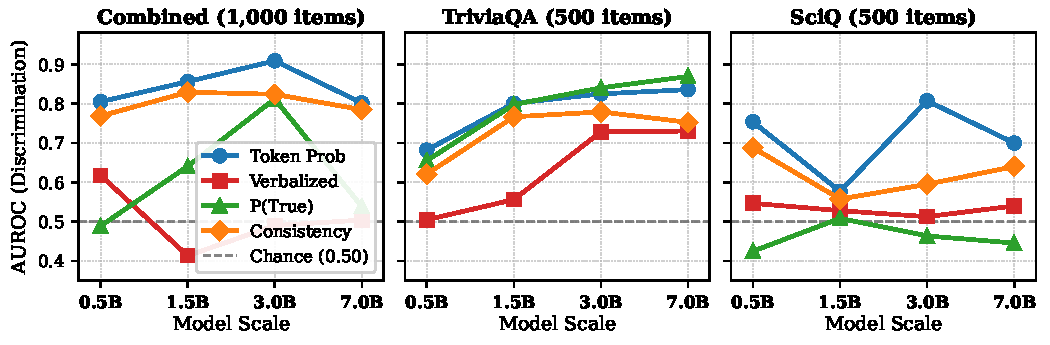
\includegraphics[width=\textwidth]{figures/fig1_auroc_vs_size.pdf}
    \caption{\textbf{Discrimination Performance (AUROC vs.\ Model Size).} Area Under the ROC Curve across model scales for four confidence estimation methods on Combined (left), TriviaQA (center), and SciQ (right). Token probability (blue) and self-consistency (orange) maintain robust discrimination across sizes, whereas verbalized confidence (red) collapses near or below random baseline (0.50).}
    \label{fig:auroc}
\end{figure*}

\begin{table*}[t]
\centering
\small
\setlength{\tabcolsep}{3.8pt}
\caption{\textbf{Comprehensive Calibration and Discrimination Benchmark.} Accuracy, AUROC ($\uparrow$), Expected Calibration Error (ECE $\downarrow$, 10 equal-width bins), and Brier Score ($\downarrow$) across Qwen2.5 models on Combined, TriviaQA, and SciQ benchmarks.}
\label{tab:metrics}
\begin{tabular}{llcccccccccc}
\toprule
& & \multicolumn{3}{c}{\textbf{Combined (N=1,000)}} & \multicolumn{3}{c}{\textbf{TriviaQA (N=500)}} & \multicolumn{3}{c}{\textbf{SciQ (N=500)}} \\
\cmidrule(lr){3-5} \cmidrule(lr){6-8} \cmidrule(lr){9-11}
\textbf{Model} & \textbf{Method} & \textbf{AUROC} $\uparrow$ & \textbf{ECE} $\downarrow$ & \textbf{Brier} $\downarrow$ & \textbf{AUROC} $\uparrow$ & \textbf{ECE} $\downarrow$ & \textbf{Brier} $\downarrow$ & \textbf{AUROC} $\uparrow$ & \textbf{ECE} $\downarrow$ & \textbf{Brier} $\downarrow$ \\
\midrule
\textbf{0.5B} & Token Prob & \textbf{0.805} & 0.331 & 0.297 & \textbf{0.682} & 0.447 & 0.338 & \textbf{0.754} & \textbf{0.215} & \textbf{0.256} \\
(Acc: 38.6\%) & Verbalized & 0.618 & 0.472 & 0.453 & 0.505 & 0.648 & 0.582 & 0.547 & 0.295 & 0.325 \\
& P(True) & 0.489 & 0.473 & 0.474 & 0.655 & 0.670 & 0.612 & 0.425 & 0.288 & 0.335 \\
& Consistency & 0.768 & \textbf{0.237} & \textbf{0.251} & 0.621 & \textbf{0.247} & \textbf{0.233} & 0.688 & 0.231 & 0.269 \\
\midrule
\textbf{1.5B} & Token Prob & \textbf{0.856} & 0.204 & 0.202 & \textbf{0.801} & 0.347 & 0.298 & \textbf{0.577} & \textbf{0.071} & \textbf{0.106} \\
(Acc: 61.8\%) & Verbalized & 0.414 & 0.338 & 0.357 & 0.556 & 0.612 & 0.604 & 0.528 & 0.083 & 0.109 \\
& P(True) & 0.641 & 0.529 & 0.537 & 0.798 & \textbf{0.190} & \textbf{0.210} & 0.508 & 0.870 & 0.863 \\
& Consistency & 0.829 & \textbf{0.162} & \textbf{0.173} & 0.766 & 0.221 & 0.240 & 0.557 & 0.105 & 0.107 \\
\midrule
\textbf{3.0B} & Token Prob & \textbf{0.909} & 0.222 & 0.198 & 0.825 & 0.380 & 0.329 & \textbf{0.807} & 0.066 & 0.066 \\
(Acc: 67.1\%) & Verbalized & 0.490 & 0.382 & 0.372 & 0.728 & 0.408 & 0.386 & 0.513 & 0.422 & 0.358 \\
& P(True) & 0.812 & 0.576 & 0.573 & \textbf{0.840} & \textbf{0.222} & \textbf{0.216} & 0.464 & 0.930 & 0.930 \\
& Consistency & 0.824 & \textbf{0.171} & \textbf{0.167} & 0.779 & 0.282 & 0.273 & 0.595 & \textbf{0.062} & \textbf{0.062} \\
\midrule
\textbf{7.0B} & Token Prob & \textbf{0.802} & \textbf{0.146} & 0.169 & 0.835 & 0.317 & 0.285 & \textbf{0.700} & \textbf{0.045} & 0.054 \\
(Acc: 73.7\%) & Verbalized & 0.504 & 0.209 & 0.271 & 0.730 & 0.309 & 0.311 & 0.540 & 0.266 & 0.232 \\
& P(True) & 0.538 & 0.571 & 0.571 & \textbf{0.869} & \textbf{0.194} & \textbf{0.196} & 0.446 & 0.944 & 0.944 \\
& Consistency & 0.785 & 0.146 & \textbf{0.154} & 0.752 & 0.247 & 0.264 & 0.640 & 0.047 & \textbf{0.046} \\
\bottomrule
\end{tabular}
\end{table*}

\subsection{Confidence Estimation Methods}
For each test item, the model first generates an answer using greedy decoding. We evaluate four confidence signals:
\begin{enumerate}
    \item \textbf{Token Probability ($c_{\text{tok}}$):} Length-normalized geometric mean of chosen tokens:
    $$c_{\text{tok}} = \exp\left( \frac{1}{N}\sum_{i=1}^N \ln p(t_i \mid t_{<i}) \right)$$
    \item \textbf{Verbalized Confidence ($c_{\text{verb}}$):} The model is prompted with the question and its greedy answer: \textit{``How confident are you that this answer is correct? Respond with only a number between 0 and 100.''} The elicited integer is divided by 100 to yield $c_{\text{verb}} \in [0, 1]$.
    \item \textbf{Self-Check P(True) ($c_{\text{ptrue}}$):} Following Kadavath et al.~\cite{kadavath2022language}, the model evaluates its own answer: \textit{``Is this answer correct? Answer True or False.''} We compute next-token probabilities over True and False tokens:
    $$c_{\text{ptrue}} = \frac{P(\text{True})}{P(\text{True}) + P(\text{False})}$$
    \item \textbf{Self-Consistency ($c_{\text{cons}}$):} We draw $K=5$ sampled generations at temperature $T=0.7$ ($\text{top\_p}=0.95$). Confidence is the fraction of sampled responses that agree with the greedy prediction ($c_{\text{cons}} \in \{0.0, 0.2, 0.4, 0.6, 0.8, 1.0\}$).
\end{enumerate}

\subsection{Evaluation Metrics}
We compute:
\begin{itemize}
    \item \textbf{AUROC} (Area Under the ROC Curve): Measures how well confidence ranks correct answers above incorrect ones (threshold-independent).
    \item \textbf{ECE} (Expected Calibration Error): Grouped into $M=10$ equal-width bins $B_m \subseteq [0, 1]$:
    $$\text{ECE} = \sum_{m=1}^{10} \frac{|B_m|}{N} \left| \text{acc}(B_m) - \text{conf}(B_m) \right|$$
    \item \textbf{Brier Score}: Mean squared error $\frac{1}{N}\sum (c_i - y_i)^2$.
\end{itemize}

\begin{figure*}[t]
    \centering
    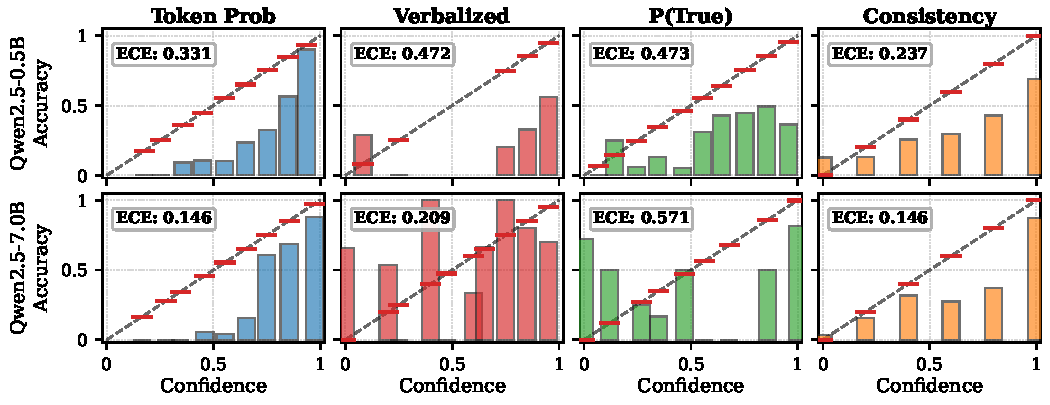
\includegraphics[width=\textwidth]{figures/fig2_reliability_diagrams.pdf}
    \caption{\textbf{Reliability Diagrams for Qwen2.5-0.5B (top) and Qwen2.5-7B (bottom).} Empirical accuracy vs.\ confidence across 10 equal bins. Dashed diagonal indicates perfect calibration. Consistency and Token Probability follow the diagonal closely, while Verbalized and P(True) suffer from extreme overconfidence and severe probability clustering.}
    \label{fig:reliability}
\end{figure*}

\section{Results and Empirical Analysis}

Table~\ref{tab:metrics} presents the complete benchmark results across all 4 models and 4 confidence methods. Figure~\ref{fig:auroc} illustrates the scaling trajectories of discrimination (AUROC).

\subsection{Task Accuracy Scaling}
Raw task performance exhibits expected scaling behavior. On combined benchmarks, accuracy rises monotonically: 38.6\% (0.5B) $\to$ 61.8\% (1.5B) $\to$ 67.1\% (3.0B) $\to$ 73.7\% (7.0B). On multiple-choice SciQ, models achieve high accuracy rapidly (60.4\% for 0.5B up to 94.4\% for 7.0B), whereas open-domain TriviaQA proves substantially more challenging (16.8\% for 0.5B up to 52.7\% for 7.0B).

\subsection{Superiority of Token Probability and Consistency}
Across all model scales, length-normalized \textbf{Token Probability} consistently delivers the highest discriminative power:
\begin{itemize}
    \item On Combined data, Token Prob achieves AUROC of \textbf{0.805} (0.5B), \textbf{0.856} (1.5B), \textbf{0.909} (3.0B), and \textbf{0.802} (7.0B).
    \item On TriviaQA open-domain generation, Token Prob AUROC increases steadily from 0.682 (0.5B) to 0.835 (7.0B).
\end{itemize}
\textbf{Self-Consistency} delivers comparable discriminative capability (Combined AUROC 0.768--0.829) while achieving the lowest calibration error across almost all configurations: ECE of 0.237 on 0.5B, dropping to \textbf{0.146} on 7.0B. Sampling 5 paths at $T=0.7$ provides an effective proxy for epistemic uncertainty.

\subsection{The Failure of Verbalized Confidence}
In sharp contrast to findings on RLHF frontier models~\cite{tian2023just}, \textbf{verbalized confidence fails catastrophically on small models}:
\begin{itemize}
    \item On Combined queries, Verbalized AUROC remains near chance level across sizes: 0.618 at 0.5B, collapsing to \textbf{0.414} at 1.5B, \textbf{0.490} at 3.0B, and \textbf{0.504} at 7.0B.
    \item In SciQ, Verbalized AUROC fluctuates between 0.513 and 0.547, showing virtually zero ability to distinguish correct choices from mistakes.
\end{itemize}
As revealed in the distribution analysis (Figure~\ref{fig:dist}), small instruction-tuned models exhibit severe mode collapse: when asked for a confidence number, models emit ``85'', ``90'', or ``95'' regardless of whether the generated answer is correct or absurdly erroneous.

\subsection{Task Dependency of Self-Check P(True)}
The self-check method $P(\text{True})$ exhibits strong domain divergence:
\begin{itemize}
    \item On \textbf{TriviaQA}, $P(\text{True})$ is remarkably effective on larger sizes, achieving the highest AUROC on 3.0B (\textbf{0.840}) and 7.0B (\textbf{0.869}) with low ECE (0.194).
    \item On \textbf{SciQ}, $P(\text{True})$ breaks down completely (AUROC 0.425--0.508, ECE $> 0.86$). When presented with a multiple-choice question and option (e.g., ``Is (A) correct?''), the model assigns high probability to ``True'' regardless of whether (A) is the correct answer, exhibiting extreme suggestibility bias~\cite{wang2025calibrating}.
\end{itemize}

\begin{figure}[t]
    \centering
    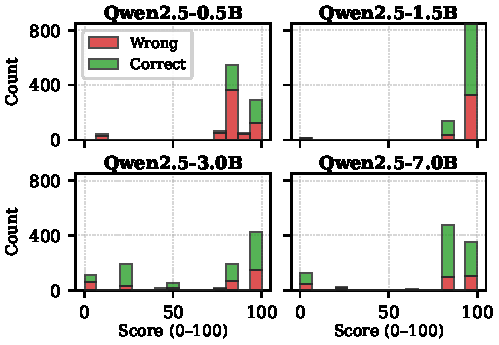
\includegraphics[width=\columnwidth]{figures/fig4_verbalized_distribution.pdf}
    \caption{\textbf{Distribution of Verbalized Confidence Scores.} Stacked histograms of verbalized scores for correct (green) vs.\ incorrect (red) answers across model scales. Small models exhibit acute mode clustering at 85--95\% with near-identical distributions for correct and incorrect answers.}
    \label{fig:dist}
\end{figure}

\section{Discussion and Limitations}
\textbf{Why Verbalization Fails in Small Models.} Small models lack the metacognitive capacity to accurately inspect internal states during post-generation prompting. Instead of reflecting certainty, the verbalization prompt triggers conversational role-play training where confident numbers are favored. Consequently, verbalization scores are almost completely uninformative.

\textbf{Practical Implications for Cascades.} In cost-saving cascades~\cite{zhang2026confidence}, routing based on verbalized confidence in small models will misroute failing queries with high confidence. Small models should exclusively route using internal token probabilities or agreement across 3--5 consistency samples.

\textbf{Limitations.} Our study was conducted within the Qwen2.5 family on two benchmark tasks. While this isolates model size as the controlled variable, future work should expand to additional architectures (e.g., Llama 3, Gemma 2) and evaluate post-hoc temperature scaling.

\section{Conclusion}
This empirical investigation evaluates confidence calibration across small open LLMs (0.5B--7B). We show that the reported superiority of verbalized confidence in large models reverses completely in small models. For small models, length-normalized token probabilities and self-consistency provide robust discrimination (AUROC up to 0.909) and calibration (ECE down to 0.146), providing a clear operational guideline for deploying small LLMs in trustworthy systems.

{\footnotesize
\let\oldbibliography\thebibliography
\renewcommand{\thebibliography}[1]{%
  \oldbibliography{#1}%
  \setlength{\itemsep}{0pt}%
  \setlength{\parskip}{0pt}%
}
\bibliographystyle{abbrv}
\bibliography{refs}
}

\end{document}
